% !TeX spellcheck = en_US
\documentclass{article}

% Pass options to natbib
\PassOptionsToPackage{numbers, compress}{natbib}

% NeurIPS packages
\usepackage[]{neurips_2023}
\usepackage[utf8]{inputenc} % allow utf-8 input
\usepackage[T1]{fontenc}    % use 8-bit T1 fonts
%\usepackage{hyperref}       % hyperlinks
\usepackage{url}            % simple URL typesetting
\usepackage{booktabs}       % professional-quality tables
\usepackage{amsfonts}       % blackboard math symbols
\usepackage{nicefrac}       % compact symbols for 1/2, etc.
\usepackage{microtype}      % microtypography
\usepackage{xcolor}         % colors

% Redefine paragraph to be tighter
\renewcommand{\paragraph}[1]{{\bf #1}~~}

% Array/table packages
\usepackage{tabularx}
\usepackage{array,multirow}
\usepackage{colortbl}
\newcommand{\PreserveBackslash}[1]{\let\temp=\\#1\let\\=\temp}
\newcolumntype{C}[1]{>{\PreserveBackslash\centering}p{#1}}
\newlength{\tblw}

% Latin
\usepackage{xspace}
\newcommand{\eg}{\textit{e.g.\@}\xspace}
\newcommand{\ie}{\textit{i.e.\@}\xspace}
\newcommand{\cf}{\textit{cf.\@}\xspace}
\newcommand{\etc}{\textit{etc.\@}\xspace}
\newcommand{\etal}{\textit{et~al.\@}\xspace}

% Our method
\newcommand{\our}{\textsc{sfr}\xspace}

% Tikz
\usepackage{tikz}
\usepackage{pgfplots}
\usetikzlibrary{patterns}
\usetikzlibrary{decorations,backgrounds,arrows.meta,calc}
\usetikzlibrary{shapes,arrows,positioning}

% Appendix/supplement title
\newcommand{\nipstitle}[1]{{%
    % rules for title box at top and bottom
    \def\toptitlebar{\hrule height4pt \vskip .25in \vskip -\parskip} 
    \def\bottomtitlebar{\vskip .29in \vskip -\parskip \hrule height1pt \vskip .09in} 
    \phantomsection\hsize\textwidth\linewidth\hsize%
    \vskip 0.1in%
    \toptitlebar%
    \begin{minipage}{\textwidth}%
        \centering{\LARGE\bf #1\par}%
    \end{minipage}%
    \bottomtitlebar%
    \addcontentsline{toc}{section}{#1}%
}}

% Bibliography
%\usepackage[maxcitenames=1, maxbibnames=4, doi=false, isbn=false, eprint=true, backend=bibtex, hyperref=true, url=false, style=authoryear-comp]{biblatex}
%\addbibresource{zotero-library.bib}
% \addbibresource{paper/zotero-library.bib}

% Let's use good old bibtex instead

% Figure customization: Tight legend box
\pgfplotsset{every axis/.append style={
		legend style={inner xsep=1pt, inner ysep=0.5pt, nodes={inner sep=1pt, text depth=0.1em},draw=none,fill=none}
}}

% Our packages
\usepackage{todonotes}
\usepackage[colorlinks=true,linkcolor=black,allcolors=black,urlcolor=black,citecolor=black]{hyperref}
\usepackage{amsmath}
\usepackage{bm}
\usepackage{algpseudocode}
\usepackage{algorithm}
\usepackage{derivative}
\usepackage{wrapfig}

\usepackage{tikz,pgfplots}
\usepackage{subcaption}
\usetikzlibrary{}

\newcommand{\defeq}{\vcentcolon=}

% Definitions/assumptions etc
\usepackage{mathtools}
\newtheorem{definition}{Definition}[section]
\newtheorem{assumption}{Assumption}[section]
\newtheorem{theorem}{Theorem}[section]
\newtheorem{lemma}{Lemma}[section]
% \newtheorem*{remark}{Remark}

% Short commands for commonly used stuff
\DeclareMathOperator{\R}{\mathbb{R}}
\DeclareMathOperator{\E}{\mathbb{E}}
\DeclareMathOperator{\V}{\mathbb{V}}


% Short section names etc
% This must be imported last!
%\usepackage{cleveref}
\usepackage[capitalise,nameinlink]{cleveref}
\crefname{section}{Sec.}{Secs.}
\crefname{algorithm}{Alg.}{Algs.}
\crefname{appendix}{App.}{Apps.}
\crefname{definition}{Def.}{Defs.}
\crefname{table}{Table}{Tables}

% Config for Arno's awesome TikZ plotting stuff
\newlength{\figurewidth}
\newlength{\figureheight}


% Variables
\newcommand{\state}{\ensuremath{\mathbf{s}}}
\newcommand{\action}{\ensuremath{\mathbf{a}}}
\newcommand{\noise}{\ensuremath{\bm\epsilon}}
\newcommand{\discount}{\ensuremath{\gamma}}
\newcommand{\inducingInput}{\ensuremath{\mathbf{Z}}}
\newcommand{\inducingVariable}{\ensuremath{\mathbf{u}}}
\newcommand{\dataset}{\ensuremath{\mathcal{D}}}
\newcommand{\dualParam}[1]{\ensuremath{\bm{\lambda}_{#1}}}
\newcommand{\meanParam}[1]{\ensuremath{\bm{\mu}_{#1}}}

% Indexes
\newcommand{\horizon}{\ensuremath{h}}
\newcommand{\Horizon}{\ensuremath{H}}
\newcommand{\numDataNew}{\ensuremath{N^{\text{new}}}}
\newcommand{\numDataOld}{\ensuremath{N^{\text{old}}}}
\newcommand{\numInducing}{\ensuremath{M}}

% Domains
\newcommand{\stateDomain}{\ensuremath{\mathcal{S}}}
\newcommand{\actionDomain}{\ensuremath{\mathcal{A}}}
\newcommand{\inputDomain}{\ensuremath{\mathbb{R}^{D}}}
\newcommand{\outputDomain}{\ensuremath{\mathbb{R}^{C}}}
\newcommand{\policyDomain}{\ensuremath{\Pi}}

% Functions
\newcommand{\rewardFn}{\ensuremath{r}}
\newcommand{\transitionFn}{\ensuremath{f}}
\newcommand{\latentFn}{\ensuremath{f}}

\newcommand{\optimisticTransition}{\ensuremath{\hat{f}}}
\newcommand{\optimisticTransitionMean}{\ensuremath{\mu_{\optimisticTransition}}}
\newcommand{\optimisticTransitionCov}{\ensuremath{\mu_{\optimisticTransition}}}
\newcommand{\optimisticTransitionSet}{\ensuremath{\mathcal{M}}}


% Parameters
% \newcommand{\weights}{\ensuremath{\bm\phi}}
\newcommand{\weights}{\ensuremath{\mathbf{w}}}
\newcommand{\valueFnParams}{\ensuremath{\psi}}
\newcommand{\policyParams}{\ensuremath{\theta}}

% Networks
\newcommand{\transitionFnWithParams}{\ensuremath{\transitionFn_{\weights}}}
\newcommand{\valueFn}{\ensuremath{\mathbf{Q}}}
\newcommand{\stateValueFn}{\ensuremath{\mathbf{V}}}
% \newcommand{\valueFn}{\ensuremath{\mathbf{Q}_{\valueFnParams}}}
\newcommand{\policy}{\ensuremath{\pi}}
\newcommand{\pPolicy}{\ensuremath{\pi_{\policyParams}}}


% Packages for bold math
\usepackage{bm}
\newcommand{\mathbold}[1]{\bm{#1}}
\newcommand{\mbf}[1]{\mathbf{#1}}
\renewcommand{\mid}{\,|\,}


% Math Macros
\newcommand{\MB}{\mbf{B}}
\newcommand{\MC}{\mbf{C}}
\newcommand{\MZ}{\mbf{Z}}
\newcommand{\MV}{\mbf{V}}
\newcommand{\MX}{\mbf{X}}
\newcommand{\MA}{\mbf{A}}
\newcommand{\MK}{\mbf{K}}
\newcommand{\MI}{\mbf{I}}
\newcommand{\MH}{\mbf{H}}
\newcommand{\T}{\top}
\newcommand{\vzeros}{\mbf{0}}
\newcommand{\vtheta}[0]{\mathbold{\theta}}
\newcommand{\valpha}[0]{\mathbold{\alpha}}
\newcommand{\vkappa}[0]{\mathbold{\kappa}}
\newcommand{\vbeta}[0]{\mathbold{\beta}}
\newcommand{\MBeta}[0]{\mathbold{B}}
\newcommand{\vlambda}[0]{\mathbold{\lambda}}
\newcommand{\diag}{\text{{diag}}}

\newcommand{\vm}{\mbf{m}}
\newcommand{\vz}{\mbf{z}}
\newcommand{\vf}{\mbf{f}}
\newcommand{\vu}{\mbf{u}}
\newcommand{\vx}{\mbf{x}}
\newcommand{\vy}{\mbf{y}}
\newcommand{\vw}{\mbf{w}}
\newcommand{\va}{\mbf{a}}

\newcommand{\Jac}[2]{\mathcal{J}_{#1}(#2)}
\newcommand{\JacT}[2]{\mathcal{J}_{#1}^\top(#2)}


\newcommand{\GP}{\mathcal{GP}}
\newcommand{\KL}[2]{\mathrm{D}_\textrm{KL} \dbar*{#1}{#2}}
\newcommand{\MKzz}{\mbf{K}_{\mbf{z}\mbf{z}}}
\newcommand{\MKzzc}{\mbf{K}_{\mbf{z}\mbf{z}, c}}
\newcommand{\MKxx}{\mbf{K}_{\mbf{x}\mbf{x}}}
\newcommand{\MKzx}{\mbf{K}_{\mbf{z}\mbf{x}}}
\newcommand{\MKxz}{\mbf{K}_{\mbf{x}\mbf{z}}}
\newcommand{\vkzi}{\mbf{k}_{\mbf{z}i}}
\newcommand{\vkzic}{\mbf{k}_{\mbf{z}i,c}}
\newcommand{\vkzs}{\mbf{k}_{\mbf{z}i}}
\newcommand{\vk}{\mbf{k}}
\newcommand{\MLambda}[0]{\mathbold{\Lambda}}
\newcommand{\MSigma}[0]{\mathbold{\Sigma}}
\definecolor{matplotlib-blue}{HTML}{1f77b4}
\newcommand{\N}{\mathrm{N}}
%\newcommand{\R}{\mathrm{R}}
\newcommand{\myexpect}{\mathbb{E}}

\DeclareMathOperator*{\argmax}{arg\,max}
\DeclareMathOperator*{\argmin}{arg\,min}
\newcommand{\Norm}{\mathcal{N}}

\newcommand{\digit}[1]{\tikz[baseline=-.5ex]\node[inner sep=1pt,rounded corners=1pt,draw=black,text width=5pt,minimum width=5pt,align=center,fill=black!20]{\tiny\bf\sf#1};}


%\title{Investigatin Uncertainty Quantification in Model-based Reinforcement Learning}
% \title{Model-based Reinforcement Learning with Fast Posterior Updates}
%\title{Sequential Decision-Making under Uncertainty with Big Data}
% \title{Neural Network to Vatiational Sparse Gaussian Process: For Adaptive Exploration}
% \title{Neural Network to Sparse Variational Gaussian Process: For Updates in Sequential Decision Making}
% \title{Adapting Neural Networks to New Data For Updates in Sequential Decision Making via Gaussian Processes}
% \title{Converting Neural Networks to Gaussian Processes for Sequential Decision-Making Under Uncertainty}
%\title{Sparse Function Space Representation of Neural Networks for Exploration and Retention}
%\title{Sparse Function-space Neural Networks}
% \title{Sparse Function-space Representation \\ of Neural Networks}% for Adaptation and Retention}
% \title{Rebuttal}% for Adaptation and Retention}
% \author{}


\begin{document}

% \maketitle


\begin{table}[t!]
  \centering\scriptsize
  \caption{Comparisons and ablations on UCI data with negative log predictive density (NLPD\textcolor{gray}{\footnotesize$\pm$std}, lower better). Our \our is generally on par with the Laplace approximation (BNN/GLM). Moreover, it performs better than the GP subset method when using a lower number of inducing points. For clarity, we specify the number of inducing points as a percent $M (\%)$ of the training data $N$.}
	\label{tbl:uci}
	%\vspace*{-4pt}

	% Control table spacing
	\renewcommand{\arraystretch}{1.}
	\setlength{\tabcolsep}{3.3pt}
	\setlength{\tblw}{0.083\textwidth}

	% Custom error formatting
	\newcommand{\val}[2]{%
		$#1$\textcolor{gray}{\tiny ${\pm}#2$}
	}

    % THE TABLE NUMBER ARE GENERATED BY A SCRIPT
	% \begin{tabular}{l C{0.6\tblw} C{0.6\tblw} C{0.6\tblw} C{0.6\tblw} C{0.6\tblw} C{0.6\tblw} C{0.6\tblw} C{0.6\tblw} C{0.6\tblw} C{0.6\tblw} C{0.6\tblw} C{0.6\tblw}}
\toprule
& NN MAP & MFVI & BNN & GLM & GLM diag & GLM refine & GLM refine d & SVGP (16) & GP subset(16) & SVGP (32) & GP subset(32)  \\
\midrule
\sc australian & \val{0.31}{0.01} & \val{0.34}{0.01} & \val{0.42}{0.0} & \val{0.32}{0.02} & \val{0.33}{0.01} & \val{0.32}{0.02} & \val{0.31}{0.01} & \val{0.322}{0.028} & \val{0.467}{0.02} & \val{0.316}{0.031} & \val{0.406}{0.016} \\
\sc cancer & \val{0.11}{0.02} & \val{0.11}{0.01} & \val{0.19}{0.0} & \val{0.1}{0.01} & \val{0.11}{0.01} & \val{0.11}{0.01} & \val{0.12}{0.02} & \val{0.102}{0.034} & \val{0.268}{0.012} & \val{0.103}{0.036} & \val{0.206}{0.017} \\
\sc ionosphere & \val{0.35}{0.02} & \val{0.41}{0.01} & \val{0.5}{0.0} & \val{0.29}{0.01} & \val{0.35}{0.01} & \val{0.35}{0.05} & \val{0.32}{0.03} & \val{0.333}{0.041} & \val{0.486}{0.02} & \val{0.313}{0.046} & \val{0.434}{0.025} \\
\sc glass & \val{0.95}{0.03} & \val{1.06}{0.01} & \val{1.41}{0.0} & \val{0.86}{0.01} & \val{0.99}{0.01} & \val{0.98}{0.07} & \val{0.83}{0.02} & \val{0.982}{0.072} & \val{1.225}{0.047} & \val{0.886}{0.082} & \val{1.086}{0.073} \\
\sc vehicle & \val{0.42}{0.007} & \val{0.504}{0.006} & \val{0.885}{0.002} & \val{0.428}{0.005} & \val{0.618}{0.003} & \val{0.402}{0.007} & \val{0.432}{0.005} & \val{0.545}{0.023} & \val{1.001}{0.024} & \val{0.51}{0.021} & \val{0.848}{0.027} \\
\sc waveform & \val{0.335}{0.004} & \val{0.393}{0.003} & \val{0.516}{0.002} & \val{0.339}{0.004} & \val{0.388}{0.003} & \val{0.335}{0.004} & \val{0.364}{0.008} & \val{0.352}{0.024} & \val{0.651}{0.009} & \val{0.343}{0.025} & \val{0.535}{0.017} \\
\sc digits & \val{0.094}{0.003} & \val{0.219}{0.004} & \val{0.875}{0.002} & \val{0.25}{0.002} & \val{0.409}{0.002} & \val{0.15}{0.002} & \val{0.149}{0.008} & \val{0.458}{0.017} & \val{1.724}{0.049} & \val{0.375}{0.015} & \val{1.394}{0.01} \\
\sc satellite & \val{0.23}{0.002} & \val{0.307}{0.002} & \val{0.482}{0.001} & \val{0.241}{0.001} & \val{0.327}{0.002} & \val{0.227}{0.002} & \val{0.248}{0.002} & \val{0}{0} & \val{0}{0} & \val{0.32}{0.013} & \val{0.827}{0.016} \\
\bottomrule
\end{tabular}

	\begin{tabular}{lcccccccc}
\toprule
 &  & \sc nn map & \sc bnn & \sc glm & {\sc gp} subset (\sc gp) & \our (\sc gp) \\
Data set & $M (\%)$ &  &  &  &  &  \\
\midrule
\multirow[t]{5}{*}{\sc Australian ($N=690, D=14, C=2$)} & 5 & - & - & - & \val{0.58}{0.06} & \val{0.36}{0.03} \\
 & 20 & - & - & - & \val{0.41}{0.04} & \val{0.35}{0.04} \\
 & 40 & - & - & - & \val{0.38}{0.03} & \val{0.35}{0.03} \\
 & 60 & - & - & - & \val{0.36}{0.04} & \val{0.35}{0.03} \\
 & - & \val{0.35}{0.06} & \val{0.34}{0.05} & \val{0.35}{0.05} & - & - \\
\cline{1-7}
\multirow[t]{5}{*}{\sc Breast cancer ($N=683, D=10, C=2$)} & 5 & - & - & - & \val{0.43}{0.22} & \val{0.08}{0.04} \\
 & 20 & - & - & - & \val{0.13}{0.03} & \val{0.08}{0.04} \\
 & 40 & - & - & - & \val{0.10}{0.04} & \val{0.08}{0.04} \\
 & 60 & - & - & - & \val{0.09}{0.04} & \val{0.08}{0.04} \\
 & - & \val{0.09}{0.05} & \val{0.09}{0.05} & \val{0.09}{0.05} & - & - \\
\cline{1-7}
\multirow[t]{5}{*}{\sc Digits ($N=1797, D=64, C=10$)} & 5 & - & - & - & \val{0.48}{0.04} & \val{0.10}{0.03} \\
 & 20 & - & - & - & \val{0.16}{0.04} & \val{0.08}{0.03} \\
 & 40 & - & - & - & \val{0.10}{0.03} & \val{0.08}{0.03} \\
 & 60 & - & - & - & \val{0.09}{0.03} & \val{0.08}{0.03} \\
 & - & \val{0.07}{0.04} & \val{0.07}{0.03} & \val{0.07}{0.04} & - & - \\
\cline{1-7}
\multirow[t]{5}{*}{\sc Glass ($N=214, D=9, C=6$)} & 5 & - & - & - & \val{1.45}{0.10} & \val{1.07}{0.10} \\
 & 20 & - & - & - & \val{1.19}{0.08} & \val{0.92}{0.11} \\
 & 40 & - & - & - & \val{1.04}{0.08} & \val{0.90}{0.13} \\
 & 60 & - & - & - & \val{0.96}{0.12} & \val{0.87}{0.17} \\
 & - & \val{1.02}{0.41} & \val{0.87}{0.28} & \val{0.82}{0.27} & - & - \\
\cline{1-7}
\multirow[t]{5}{*}{\sc Ionosphere ($N=351, D=34, C=2$)} & 5 & - & - & - & \val{0.63}{0.05} & \val{0.39}{0.04} \\
 & 20 & - & - & - & \val{0.44}{0.03} & \val{0.39}{0.04} \\
 & 40 & - & - & - & \val{0.41}{0.03} & \val{0.39}{0.04} \\
 & 60 & - & - & - & \val{0.41}{0.06} & \val{0.38}{0.04} \\
 & - & \val{0.38}{0.05} & \val{0.38}{0.05} & \val{0.37}{0.05} & - & - \\
\cline{1-7}
\multirow[t]{5}{*}{\sc Satellite ($N=6435, D=35, C=6$)} & 5 & - & - & - & \val{0.72}{0.02} & \val{0.31}{0.02} \\
 & 20 & - & - & - & \val{0.43}{0.05} & \val{0.31}{0.03} \\
 & 40 & - & - & - & \val{0.39}{0.04} & \val{0.30}{0.02} \\
 & 60 & - & - & - & \val{0.35}{0.03} & \val{0.30}{0.02} \\
 & - & \val{0.24}{0.02} & \val{0.24}{0.02} & \val{0.24}{0.02} & - & - \\
\cline{1-7}
\multirow[t]{5}{*}{\sc Vehicle ($N=846, D=18, C=4$)} & 5 & - & - & - & \val{1.09}{0.23} & \val{0.47}{0.03} \\
 & 20 & - & - & - & \val{0.61}{0.06} & \val{0.43}{0.02} \\
 & 40 & - & - & - & \val{0.49}{0.04} & \val{0.43}{0.03} \\
 & 60 & - & - & - & \val{0.45}{0.01} & \val{0.44}{0.02} \\
 & - & \val{0.40}{0.06} & \val{0.38}{0.06} & \val{0.37}{0.04} & - & - \\
\cline{1-7}
\multirow[t]{5}{*}{\sc Waveform ($N=1000, D=21, C=3$)} & 5 & - & - & - & \val{0.61}{0.24} & \val{0.33}{0.03} \\
 & 20 & - & - & - & \val{0.36}{0.03} & \val{0.32}{0.03} \\
 & 40 & - & - & - & \val{0.33}{0.03} & \val{0.32}{0.03} \\
 & 60 & - & - & - & \val{0.32}{0.03} & \val{0.32}{0.03} \\
 & - & \val{0.40}{0.05} & \val{0.35}{0.04} & \val{0.36}{0.03} & - & - \\
\bottomrule
\end{tabular}

\end{table}

%
\begin{figure}[t]
  \centering\scriptsize
  \setlength{\figurewidth}{.26\textwidth}
  \setlength{\figureheight}{\figurewidth}
  \pgfplotsset{axis on top,scale only axis,y tick label style={rotate=90}, x tick label style={font=\footnotesize},y tick label style={font=\footnotesize},title style={yshift=-4pt,font=\large}, y label style={font=\large},x label style={font=\large},grid=major, width=\figurewidth, height=\figureheight}
  % \pgfplotsset{axis on top,scale only axis,y tick label style={rotate=90}, x tick label style={font=\footnotesize},y tick label style={font=\footnotesize},title style={yshift=-4pt,font=\large}, y label style={font=\large},x label style={font=\large},grid=major, width=\figurewidth, height=\figureheight}
  \pgfplotsset{grid style={line width=.1pt, draw=gray!10,dashed}}
  \pgfplotsset{xlabel={$M$ as \% of $N$},ylabel style={yshift=-12pt}}
  %
  \begin{minipage}[t]{.16\textwidth}
    \raggedleft
    \pgfplotsset{ylabel=NLPD}
    % This file was created by tikzplotlib v0.9.8.
\begin{tikzpicture}

\definecolor{color0}{rgb}{0.274509803921569,0.509803921568627,0.705882352941177}
\definecolor{color1}{rgb}{1,0.549019607843137,0}

\begin{axis}[
height=\figureheight,
tick align=outside,
tick pos=left,
width=\figurewidth,
x grid style={white!69.0196078431373!black},
xlabel={\(\displaystyle M\) as \% of N},
xmin=-5, xmax=105,
xtick style={color=black},
xtick={-20,0,20,40,60,80,100,120},
xticklabels={\ensuremath{-}20,0,20,40,60,80,100,120},
y grid style={white!69.0196078431373!black},
ylabel={NLPD},
ymin=0.295205354934127, ymax=0.711423720917342,
ytick style={color=black},
ytick={0.2,0.4,0.6,0.8},
yticklabels={0.2,0.4,0.6,0.8}
]
\path [draw=color0, fill=color0, opacity=0.1]
(axis cs:1,0.494221211965826)
--(axis cs:1,0.399321652492671)
--(axis cs:2,0.351059794088986)
--(axis cs:5,0.320472089061091)
--(axis cs:10,0.325467508462525)
--(axis cs:15,0.325597490738425)
--(axis cs:20,0.319012120906293)
--(axis cs:40,0.321316936554183)
--(axis cs:60,0.319776159569208)
--(axis cs:80,0.325610068775334)
--(axis cs:100,0.314124371569727)
--(axis cs:100,0.37706293427259)
--(axis cs:100,0.37706293427259)
--(axis cs:80,0.380206902276773)
--(axis cs:60,0.374746105543953)
--(axis cs:40,0.373502864764141)
--(axis cs:20,0.378346982386726)
--(axis cs:15,0.372088416139428)
--(axis cs:10,0.372775164916083)
--(axis cs:5,0.38023494105999)
--(axis cs:2,0.392444030893242)
--(axis cs:1,0.494221211965826)
--cycle;

\path [draw=color1, fill=color1, opacity=0.1]
(axis cs:1,0.687448930777529)
--(axis cs:1,0.651722955032714)
--(axis cs:2,0.640662185338724)
--(axis cs:5,0.552349369369992)
--(axis cs:10,0.457703698540147)
--(axis cs:15,0.445415377639606)
--(axis cs:20,0.416635028643809)
--(axis cs:40,0.367666345547475)
--(axis cs:60,0.358534351547199)
--(axis cs:80,0.326042220369126)
--(axis cs:100,0.320320042731056)
--(axis cs:100,0.370067114309538)
--(axis cs:100,0.370067114309538)
--(axis cs:80,0.379197253443171)
--(axis cs:60,0.38209219531885)
--(axis cs:40,0.407522537225998)
--(axis cs:20,0.463360216623672)
--(axis cs:15,0.468843270336541)
--(axis cs:10,0.494496186276123)
--(axis cs:5,0.598263927796181)
--(axis cs:2,0.692504704281741)
--(axis cs:1,0.687448930777529)
--cycle;

\addplot [semithick, color0]
table {%
1 0.446771432229249
2 0.371751912491114
5 0.35035351506054
10 0.349121336689304
15 0.348842953438926
20 0.34867955164651
40 0.347409900659162
60 0.34726113255658
80 0.352908485526053
100 0.345593652921159
};
\addplot [semithick, color1]
table {%
1 0.669585942905121
2 0.666583444810232
5 0.575306648583086
10 0.476099942408135
15 0.457129323988073
20 0.439997622633741
40 0.387594441386737
60 0.370313273433025
80 0.352619736906148
100 0.345193578520297
};
\end{axis}

\end{tikzpicture}

  \end{minipage}
  \hfill
%  \begin{minipage}[t]{.16\textwidth}
%    \raggedleft
%    % This file was created with tikzplotlib v0.10.1.
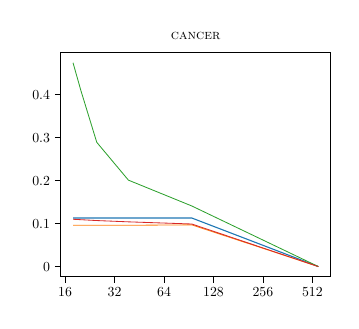
\begin{tikzpicture}[
scale=0.5
]

\definecolor{crimson2143940}{RGB}{214,39,40}
\definecolor{darkgray176}{RGB}{176,176,176}
\definecolor{darkorange25512714}{RGB}{255,127,14}
\definecolor{forestgreen4416044}{RGB}{44,160,44}
\definecolor{steelblue31119180}{RGB}{31,119,180}

\begin{axis}[
tick align=outside,
tick pos=left,
title={\sc cancer},
x grid style={darkgray176},
xmin=-8.8, xmax=536.8,
xtick style={color=black},
xtick={-100,0,100,200,300,400,500,600},
xticklabels={0,16,32,64,128,256,512,},
y grid style={darkgray176},
ymin=-0.0237, ymax=0.4977,
ytick style={color=black}
]
\addplot [thick, steelblue31119180]
table {%
16 0.113
32 0.113
64 0.113
128 0.113
256 0.113
512 0
};
\addplot [semithick, darkorange25512714]
table {%
16 0.096
32 0.096
64 0.096
128 0.096
256 0.097
512 0
};
\addplot [semithick, forestgreen4416044]
table {%
16 0.474
32 0.409
64 0.289
128 0.201
256 0.141
512 0
};
\addplot [semithick, crimson2143940]
table {%
16 0.11
32 0.109
64 0.107
128 0.104
256 0.099
512 0
};
\end{axis}

\end{tikzpicture}

%  \end{minipage}
%  \hfill
%  \begin{minipage}[t]{.16\textwidth}
%    \raggedleft
%    % This file was created with tikzplotlib v0.10.1.
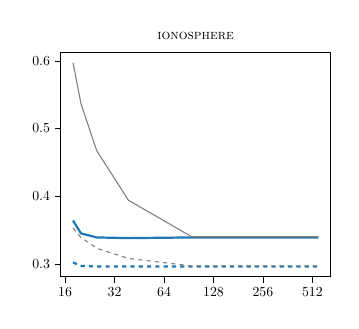
\begin{tikzpicture}[
scale=0.5
]

\definecolor{darkgray176}{RGB}{176,176,176}
\definecolor{gray}{RGB}{128,128,128}
\definecolor{steelblue31119180}{RGB}{31,119,180}

\begin{axis}[
tick align=outside,
tick pos=left,
title={\sc ionosphere},
x grid style={darkgray176},
xmin=-8.8, xmax=536.8,
xtick style={color=black},
xtick={-100,0,100,200,300,400,500,600},
xticklabels={0,16,32,64,128,256,512,},
y grid style={darkgray176},
ymin=0.28095, ymax=0.61205,
ytick style={color=black}
]
\addplot [ultra thick, steelblue31119180]
table {%
16 0.364
32 0.345
64 0.339
128 0.338
256 0.339
512 0.339
};
\addplot [ultra thick, steelblue31119180, dashed]
table {%
16 0.302
32 0.297
64 0.296
128 0.296
256 0.296
512 0.296
};
\addplot [thick, gray]
table {%
16 0.597
32 0.537
64 0.467
128 0.394
256 0.34
512 0.34
};
\addplot [thick, gray, dashed]
table {%
16 0.353
32 0.339
64 0.323
128 0.308
256 0.297
512 0.297
};
\end{axis}

\end{tikzpicture}

%  \end{minipage}
%  \hfill
  \begin{minipage}[t]{.16\textwidth}
    \raggedleft
    % This file was created by tikzplotlib v0.9.8.
\begin{tikzpicture}[scale=0.5]

\definecolor{color0}{rgb}{0.274509803921569,0.509803921568627,0.705882352941177}
\definecolor{color1}{rgb}{1,0.549019607843137,0}

\begin{axis}[
height=\figureheight,
tick align=outside,
tick pos=left,
title={\sc{Glass}},
width=\figurewidth,
x grid style={white!69.0196078431373!black},
xmin=-5, xmax=105,
xtick style={color=black},
xtick={-20,0,20,40,60,80,100,120},
xticklabels={\ensuremath{-}20,0,20,40,60,80,100,120},
y grid style={white!69.0196078431373!black},
ymin=0.645730930143993, ymax=1.81802513016566,
ytick style={color=black}
]
\path [draw=color0, fill=color0, opacity=0.1]
(axis cs:1,1.49771547138196)
--(axis cs:1,1.18952652316133)
--(axis cs:1,1.18266373930492)
--(axis cs:5,0.96605549198983)
--(axis cs:9,0.857698870422498)
--(axis cs:15,0.78946981593607)
--(axis cs:19,0.809266568098092)
--(axis cs:39,0.762809039558936)
--(axis cs:59,0.699017030144978)
--(axis cs:79,0.729237532733376)
--(axis cs:99,0.720662924824656)
--(axis cs:99,1.04896167752313)
--(axis cs:99,1.04896167752313)
--(axis cs:79,0.995374423453727)
--(axis cs:59,1.0311643117542)
--(axis cs:39,1.02993831156299)
--(axis cs:19,1.03639284358281)
--(axis cs:15,1.04105346761967)
--(axis cs:9,1.02568275842161)
--(axis cs:5,1.16679810278829)
--(axis cs:1,1.35410828283228)
--(axis cs:1,1.49771547138196)
--cycle;

\path [draw=color1, fill=color1, opacity=0.1]
(axis cs:1,1.76473903016467)
--(axis cs:1,1.58753965664686)
--(axis cs:1,1.57139842233233)
--(axis cs:5,1.35246612424739)
--(axis cs:9,1.24713571688454)
--(axis cs:15,1.14321333399575)
--(axis cs:19,1.11838605334277)
--(axis cs:39,0.956363946082652)
--(axis cs:59,0.843593507041992)
--(axis cs:79,0.782856534900766)
--(axis cs:99,0.743711704977892)
--(axis cs:99,1.01490281645003)
--(axis cs:99,1.01490281645003)
--(axis cs:79,1.04688512529527)
--(axis cs:59,1.08499783743299)
--(axis cs:39,1.12512608223656)
--(axis cs:19,1.27061408651308)
--(axis cs:15,1.26826043220348)
--(axis cs:9,1.56711712146726)
--(axis cs:5,1.55216843320769)
--(axis cs:1,1.6887418957198)
--(axis cs:1,1.76473903016467)
--cycle;

\addplot [semithick, color0]
table {%
1 1.34362099727164
1 1.2683860110686
5 1.06642679738906
9 0.941690814422055
15 0.915261641777871
19 0.922829705840453
39 0.896373675560965
59 0.865090670949587
79 0.862305978093552
99 0.884812301173894
};
\addplot [semithick, color1]
table {%
1 1.67613934340577
1 1.63007015902607
5 1.45231727872754
9 1.4071264191759
15 1.20573688309961
19 1.19450006992792
39 1.0407450141596
59 0.96429567223749
79 0.914870830098019
99 0.879307260713959
};
\end{axis}

\end{tikzpicture}

  \end{minipage}
  \hfill
  \begin{minipage}[t]{.16\textwidth}
    \raggedleft
    % This file was created with tikzplotlib v0.10.1.
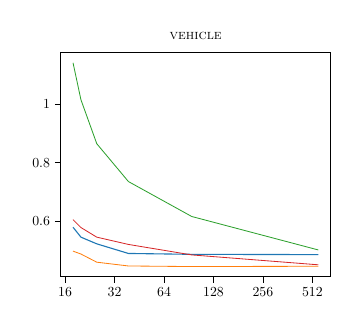
\begin{tikzpicture}[
scale=0.5
]

\definecolor{crimson2143940}{RGB}{214,39,40}
\definecolor{darkgray176}{RGB}{176,176,176}
\definecolor{darkorange25512714}{RGB}{255,127,14}
\definecolor{forestgreen4416044}{RGB}{44,160,44}
\definecolor{steelblue31119180}{RGB}{31,119,180}

\begin{axis}[
tick align=outside,
tick pos=left,
title={\sc vehicle},
x grid style={darkgray176},
xmin=-8.8, xmax=536.8,
xtick style={color=black},
xtick={-100,0,100,200,300,400,500,600},
xticklabels={0,16,32,64,128,256,512,},
y grid style={darkgray176},
ymin=0.408, ymax=1.178,
ytick style={color=black}
]
\addplot [thick, steelblue31119180]
table {%
16 0.578
32 0.544
64 0.521
128 0.488
256 0.485
512 0.484
};
\addplot [semithick, darkorange25512714]
table {%
16 0.496
32 0.486
64 0.458
128 0.445
256 0.443
512 0.444
};
\addplot [semithick, forestgreen4416044]
table {%
16 1.143
32 1.016
64 0.865
128 0.735
256 0.615
512 0.5
};
\addplot [semithick, crimson2143940]
table {%
16 0.604
32 0.577
64 0.544
128 0.519
256 0.483
512 0.449
};
\end{axis}

\end{tikzpicture}

  \end{minipage}
  \hfill
  \begin{minipage}[t]{.16\textwidth}
    \raggedleft
    % This file was created with tikzplotlib v0.10.1.
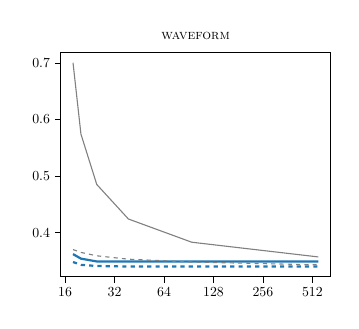
\begin{tikzpicture}[
scale=0.5
]

\definecolor{darkgray176}{RGB}{176,176,176}
\definecolor{gray}{RGB}{128,128,128}
\definecolor{steelblue31119180}{RGB}{31,119,180}

\begin{axis}[
tick align=outside,
tick pos=left,
title={\sc waveform},
x grid style={darkgray176},
xmin=-8.8, xmax=536.8,
xtick style={color=black},
xtick={-100,0,100,200,300,400,500,600},
xticklabels={0,16,32,64,128,256,512,},
y grid style={darkgray176},
ymin=0.322, ymax=0.718,
ytick style={color=black}
]
\addplot [ultra thick, steelblue31119180]
table {%
16 0.362
32 0.354
64 0.349
128 0.349
256 0.349
512 0.349
};
\addplot [ultra thick, steelblue31119180, dashed]
table {%
16 0.348
32 0.343
64 0.341
128 0.34
256 0.34
512 0.34
};
\addplot [thick, gray]
table {%
16 0.7
32 0.574
64 0.485
128 0.424
256 0.383
512 0.357
};
\addplot [thick, gray, dashed]
table {%
16 0.37
32 0.365
64 0.359
128 0.353
256 0.348
512 0.343
};
\end{axis}

\end{tikzpicture}

  \end{minipage}
  \hfill
  \begin{minipage}[t]{.16\textwidth}
    \raggedleft
    % This file was created with tikzplotlib v0.10.1.
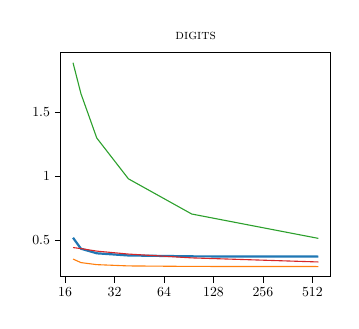
\begin{tikzpicture}[
scale=0.5
]

\definecolor{crimson2143940}{RGB}{214,39,40}
\definecolor{darkgray176}{RGB}{176,176,176}
\definecolor{darkorange25512714}{RGB}{255,127,14}
\definecolor{forestgreen4416044}{RGB}{44,160,44}
\definecolor{steelblue31119180}{RGB}{31,119,180}

\begin{axis}[
tick align=outside,
tick pos=left,
title={\sc digits},
x grid style={darkgray176},
xmin=-8.8, xmax=536.8,
xtick style={color=black},
xtick={-100,0,100,200,300,400,500,600},
xticklabels={0,16,32,64,128,256,512,},
y grid style={darkgray176},
ymin=0.2101, ymax=1.9679,
ytick style={color=black}
]
\addplot [ultra thick, steelblue31119180]
table {%
16 0.516
32 0.43
64 0.394
128 0.377
256 0.37
512 0.368
};
\addplot [thick, darkorange25512714]
table {%
16 0.349
32 0.321
64 0.305
128 0.295
256 0.291
512 0.29
};
\addplot [thick, forestgreen4416044]
table {%
16 1.888
32 1.646
64 1.298
128 0.978
256 0.702
512 0.511
};
\addplot [thick, crimson2143940]
table {%
16 0.439
32 0.431
64 0.411
128 0.388
256 0.358
512 0.326
};
\end{axis}

\end{tikzpicture}

  \end{minipage}
  \hfill
  \begin{minipage}[t]{.16\textwidth}
    \raggedleft
    % This file was created with tikzplotlib v0.10.1.
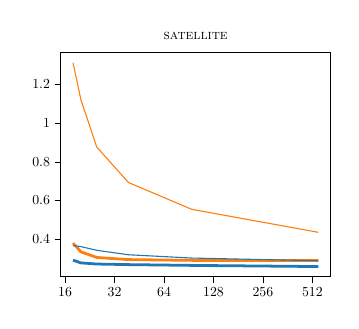
\begin{tikzpicture}[
scale=0.5
]

\definecolor{darkgray176}{RGB}{176,176,176}
\definecolor{darkorange25512714}{RGB}{255,127,14}
\definecolor{steelblue31119180}{RGB}{31,119,180}

\begin{axis}[
tick align=outside,
tick pos=left,
title={\sc satellite},
x grid style={darkgray176},
xmin=-8.8, xmax=536.8,
xtick style={color=black},
xtick={-100,0,100,200,300,400,500,600},
xticklabels={0,16,32,64,128,256,512,},
y grid style={darkgray176},
ymin=0.2053, ymax=1.3647,
ytick style={color=black}
]
\addplot [line width=2pt, darkorange25512714]
table {%
16 0.379
32 0.334
64 0.305
128 0.294
256 0.29
512 0.289
};
\addplot [line width=2pt, steelblue31119180]
table {%
16 0.291
32 0.277
64 0.271
128 0.268
256 0.264
512 0.258
};
\addplot [thick, darkorange25512714]
table {%
16 1.312
32 1.12
64 0.876
128 0.693
256 0.554
512 0.435
};
\addplot [thick, steelblue31119180]
table {%
16 0.367
32 0.361
64 0.342
128 0.319
256 0.302
512 0.288
};
\end{axis}

\end{tikzpicture}

  \end{minipage}\\[-1em]
  %
  % Legend
  \definecolor{steelblue31119180}{RGB}{31,119,180}
  \definecolor{darkorange25512714}{RGB}{255,127,14}
  \newcommand{\myline}[1]{\protect\tikz[baseline=-.5ex,line width=1.6pt]\protect\draw[draw=#1](0,0)--(1.2em,0);}
  \caption{Comparison of convergence in terms of number of inducing points $M$ in NLPD (mean over 5 seeds) on UCI classification tasks: \our (GP) (\myline{steelblue31119180}) vs.\ GP subset (GP) (\myline{darkorange25512714}). Our \our (GP) converges fast for all cases.\looseness-1}
  \label{fig:uci}
  %\vspace*{-6pt}
\end{figure}


% \section{Old (won't be in rebuttal, just for our reference)}

\end{document}


\clearpage

\begin{figure}
  \centering\scriptsize
  \setlength{\figurewidth}{.26\textwidth}
  \setlength{\figureheight}{\figurewidth}
  \pgfplotsset{axis on top,scale only axis,y tick label style={rotate=90}, x tick label style={font=\footnotesize},y tick label style={font=\footnotesize},title style={yshift=-4pt,font=\large}, y label style={font=\large},x label style={font=\large},grid=major, width=\figurewidth, height=\figureheight}
  \pgfplotsset{grid style={line width=.1pt, draw=gray!10,dashed}}
  \pgfplotsset{xlabel={$M$},ylabel style={yshift=-12pt}}
  %
  \begin{minipage}[t]{.17\textwidth}
    \raggedleft
    \pgfplotsset{ylabel=NLPD}
    % This file was created by tikzplotlib v0.9.8.
\begin{tikzpicture}

\definecolor{color0}{rgb}{0.274509803921569,0.509803921568627,0.705882352941177}
\definecolor{color1}{rgb}{1,0.549019607843137,0}

\begin{axis}[
height=\figureheight,
tick align=outside,
tick pos=left,
width=\figurewidth,
x grid style={white!69.0196078431373!black},
xlabel={\(\displaystyle M\) as \% of N},
xmin=-5, xmax=105,
xtick style={color=black},
xtick={-20,0,20,40,60,80,100,120},
xticklabels={\ensuremath{-}20,0,20,40,60,80,100,120},
y grid style={white!69.0196078431373!black},
ylabel={NLPD},
ymin=0.295205354934127, ymax=0.711423720917342,
ytick style={color=black},
ytick={0.2,0.4,0.6,0.8},
yticklabels={0.2,0.4,0.6,0.8}
]
\path [draw=color0, fill=color0, opacity=0.1]
(axis cs:1,0.494221211965826)
--(axis cs:1,0.399321652492671)
--(axis cs:2,0.351059794088986)
--(axis cs:5,0.320472089061091)
--(axis cs:10,0.325467508462525)
--(axis cs:15,0.325597490738425)
--(axis cs:20,0.319012120906293)
--(axis cs:40,0.321316936554183)
--(axis cs:60,0.319776159569208)
--(axis cs:80,0.325610068775334)
--(axis cs:100,0.314124371569727)
--(axis cs:100,0.37706293427259)
--(axis cs:100,0.37706293427259)
--(axis cs:80,0.380206902276773)
--(axis cs:60,0.374746105543953)
--(axis cs:40,0.373502864764141)
--(axis cs:20,0.378346982386726)
--(axis cs:15,0.372088416139428)
--(axis cs:10,0.372775164916083)
--(axis cs:5,0.38023494105999)
--(axis cs:2,0.392444030893242)
--(axis cs:1,0.494221211965826)
--cycle;

\path [draw=color1, fill=color1, opacity=0.1]
(axis cs:1,0.687448930777529)
--(axis cs:1,0.651722955032714)
--(axis cs:2,0.640662185338724)
--(axis cs:5,0.552349369369992)
--(axis cs:10,0.457703698540147)
--(axis cs:15,0.445415377639606)
--(axis cs:20,0.416635028643809)
--(axis cs:40,0.367666345547475)
--(axis cs:60,0.358534351547199)
--(axis cs:80,0.326042220369126)
--(axis cs:100,0.320320042731056)
--(axis cs:100,0.370067114309538)
--(axis cs:100,0.370067114309538)
--(axis cs:80,0.379197253443171)
--(axis cs:60,0.38209219531885)
--(axis cs:40,0.407522537225998)
--(axis cs:20,0.463360216623672)
--(axis cs:15,0.468843270336541)
--(axis cs:10,0.494496186276123)
--(axis cs:5,0.598263927796181)
--(axis cs:2,0.692504704281741)
--(axis cs:1,0.687448930777529)
--cycle;

\addplot [semithick, color0]
table {%
1 0.446771432229249
2 0.371751912491114
5 0.35035351506054
10 0.349121336689304
15 0.348842953438926
20 0.34867955164651
40 0.347409900659162
60 0.34726113255658
80 0.352908485526053
100 0.345593652921159
};
\addplot [semithick, color1]
table {%
1 0.669585942905121
2 0.666583444810232
5 0.575306648583086
10 0.476099942408135
15 0.457129323988073
20 0.439997622633741
40 0.387594441386737
60 0.370313273433025
80 0.352619736906148
100 0.345193578520297
};
\end{axis}

\end{tikzpicture}

  \end{minipage}
  \hfill
%  \begin{minipage}[t]{.16\textwidth}
%    \raggedleft
%    % This file was created with tikzplotlib v0.10.1.
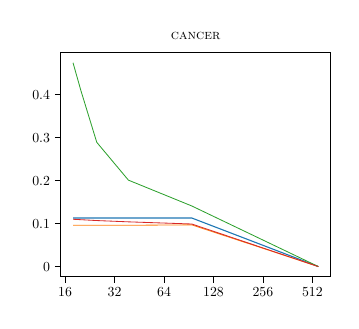
\begin{tikzpicture}[
scale=0.5
]

\definecolor{crimson2143940}{RGB}{214,39,40}
\definecolor{darkgray176}{RGB}{176,176,176}
\definecolor{darkorange25512714}{RGB}{255,127,14}
\definecolor{forestgreen4416044}{RGB}{44,160,44}
\definecolor{steelblue31119180}{RGB}{31,119,180}

\begin{axis}[
tick align=outside,
tick pos=left,
title={\sc cancer},
x grid style={darkgray176},
xmin=-8.8, xmax=536.8,
xtick style={color=black},
xtick={-100,0,100,200,300,400,500,600},
xticklabels={0,16,32,64,128,256,512,},
y grid style={darkgray176},
ymin=-0.0237, ymax=0.4977,
ytick style={color=black}
]
\addplot [thick, steelblue31119180]
table {%
16 0.113
32 0.113
64 0.113
128 0.113
256 0.113
512 0
};
\addplot [semithick, darkorange25512714]
table {%
16 0.096
32 0.096
64 0.096
128 0.096
256 0.097
512 0
};
\addplot [semithick, forestgreen4416044]
table {%
16 0.474
32 0.409
64 0.289
128 0.201
256 0.141
512 0
};
\addplot [semithick, crimson2143940]
table {%
16 0.11
32 0.109
64 0.107
128 0.104
256 0.099
512 0
};
\end{axis}

\end{tikzpicture}

%  \end{minipage}
%  \hfill
%  \begin{minipage}[t]{.16\textwidth}
%    \raggedleft
%    % This file was created with tikzplotlib v0.10.1.
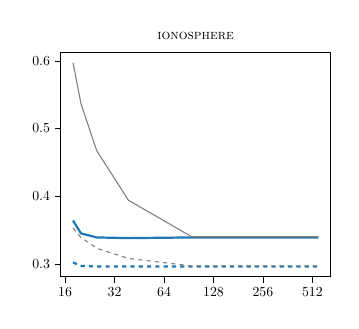
\begin{tikzpicture}[
scale=0.5
]

\definecolor{darkgray176}{RGB}{176,176,176}
\definecolor{gray}{RGB}{128,128,128}
\definecolor{steelblue31119180}{RGB}{31,119,180}

\begin{axis}[
tick align=outside,
tick pos=left,
title={\sc ionosphere},
x grid style={darkgray176},
xmin=-8.8, xmax=536.8,
xtick style={color=black},
xtick={-100,0,100,200,300,400,500,600},
xticklabels={0,16,32,64,128,256,512,},
y grid style={darkgray176},
ymin=0.28095, ymax=0.61205,
ytick style={color=black}
]
\addplot [ultra thick, steelblue31119180]
table {%
16 0.364
32 0.345
64 0.339
128 0.338
256 0.339
512 0.339
};
\addplot [ultra thick, steelblue31119180, dashed]
table {%
16 0.302
32 0.297
64 0.296
128 0.296
256 0.296
512 0.296
};
\addplot [thick, gray]
table {%
16 0.597
32 0.537
64 0.467
128 0.394
256 0.34
512 0.34
};
\addplot [thick, gray, dashed]
table {%
16 0.353
32 0.339
64 0.323
128 0.308
256 0.297
512 0.297
};
\end{axis}

\end{tikzpicture}

%  \end{minipage}
%  \hfill
  \begin{minipage}[t]{.16\textwidth}
    \raggedleft
    % This file was created by tikzplotlib v0.9.8.
\begin{tikzpicture}[scale=0.5]

\definecolor{color0}{rgb}{0.274509803921569,0.509803921568627,0.705882352941177}
\definecolor{color1}{rgb}{1,0.549019607843137,0}

\begin{axis}[
height=\figureheight,
tick align=outside,
tick pos=left,
title={\sc{Glass}},
width=\figurewidth,
x grid style={white!69.0196078431373!black},
xmin=-5, xmax=105,
xtick style={color=black},
xtick={-20,0,20,40,60,80,100,120},
xticklabels={\ensuremath{-}20,0,20,40,60,80,100,120},
y grid style={white!69.0196078431373!black},
ymin=0.645730930143993, ymax=1.81802513016566,
ytick style={color=black}
]
\path [draw=color0, fill=color0, opacity=0.1]
(axis cs:1,1.49771547138196)
--(axis cs:1,1.18952652316133)
--(axis cs:1,1.18266373930492)
--(axis cs:5,0.96605549198983)
--(axis cs:9,0.857698870422498)
--(axis cs:15,0.78946981593607)
--(axis cs:19,0.809266568098092)
--(axis cs:39,0.762809039558936)
--(axis cs:59,0.699017030144978)
--(axis cs:79,0.729237532733376)
--(axis cs:99,0.720662924824656)
--(axis cs:99,1.04896167752313)
--(axis cs:99,1.04896167752313)
--(axis cs:79,0.995374423453727)
--(axis cs:59,1.0311643117542)
--(axis cs:39,1.02993831156299)
--(axis cs:19,1.03639284358281)
--(axis cs:15,1.04105346761967)
--(axis cs:9,1.02568275842161)
--(axis cs:5,1.16679810278829)
--(axis cs:1,1.35410828283228)
--(axis cs:1,1.49771547138196)
--cycle;

\path [draw=color1, fill=color1, opacity=0.1]
(axis cs:1,1.76473903016467)
--(axis cs:1,1.58753965664686)
--(axis cs:1,1.57139842233233)
--(axis cs:5,1.35246612424739)
--(axis cs:9,1.24713571688454)
--(axis cs:15,1.14321333399575)
--(axis cs:19,1.11838605334277)
--(axis cs:39,0.956363946082652)
--(axis cs:59,0.843593507041992)
--(axis cs:79,0.782856534900766)
--(axis cs:99,0.743711704977892)
--(axis cs:99,1.01490281645003)
--(axis cs:99,1.01490281645003)
--(axis cs:79,1.04688512529527)
--(axis cs:59,1.08499783743299)
--(axis cs:39,1.12512608223656)
--(axis cs:19,1.27061408651308)
--(axis cs:15,1.26826043220348)
--(axis cs:9,1.56711712146726)
--(axis cs:5,1.55216843320769)
--(axis cs:1,1.6887418957198)
--(axis cs:1,1.76473903016467)
--cycle;

\addplot [semithick, color0]
table {%
1 1.34362099727164
1 1.2683860110686
5 1.06642679738906
9 0.941690814422055
15 0.915261641777871
19 0.922829705840453
39 0.896373675560965
59 0.865090670949587
79 0.862305978093552
99 0.884812301173894
};
\addplot [semithick, color1]
table {%
1 1.67613934340577
1 1.63007015902607
5 1.45231727872754
9 1.4071264191759
15 1.20573688309961
19 1.19450006992792
39 1.0407450141596
59 0.96429567223749
79 0.914870830098019
99 0.879307260713959
};
\end{axis}

\end{tikzpicture}

  \end{minipage}
  \hfill
  \begin{minipage}[t]{.16\textwidth}
    \raggedleft
    % This file was created with tikzplotlib v0.10.1.
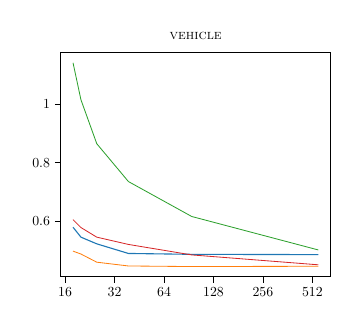
\begin{tikzpicture}[
scale=0.5
]

\definecolor{crimson2143940}{RGB}{214,39,40}
\definecolor{darkgray176}{RGB}{176,176,176}
\definecolor{darkorange25512714}{RGB}{255,127,14}
\definecolor{forestgreen4416044}{RGB}{44,160,44}
\definecolor{steelblue31119180}{RGB}{31,119,180}

\begin{axis}[
tick align=outside,
tick pos=left,
title={\sc vehicle},
x grid style={darkgray176},
xmin=-8.8, xmax=536.8,
xtick style={color=black},
xtick={-100,0,100,200,300,400,500,600},
xticklabels={0,16,32,64,128,256,512,},
y grid style={darkgray176},
ymin=0.408, ymax=1.178,
ytick style={color=black}
]
\addplot [thick, steelblue31119180]
table {%
16 0.578
32 0.544
64 0.521
128 0.488
256 0.485
512 0.484
};
\addplot [semithick, darkorange25512714]
table {%
16 0.496
32 0.486
64 0.458
128 0.445
256 0.443
512 0.444
};
\addplot [semithick, forestgreen4416044]
table {%
16 1.143
32 1.016
64 0.865
128 0.735
256 0.615
512 0.5
};
\addplot [semithick, crimson2143940]
table {%
16 0.604
32 0.577
64 0.544
128 0.519
256 0.483
512 0.449
};
\end{axis}

\end{tikzpicture}

  \end{minipage}
  \hfill
  \begin{minipage}[t]{.16\textwidth}
    \raggedleft
    % This file was created with tikzplotlib v0.10.1.
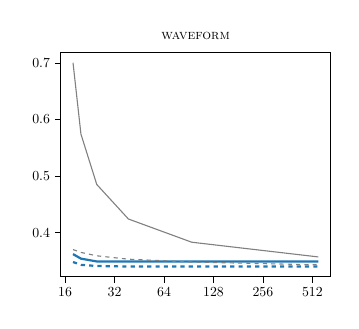
\begin{tikzpicture}[
scale=0.5
]

\definecolor{darkgray176}{RGB}{176,176,176}
\definecolor{gray}{RGB}{128,128,128}
\definecolor{steelblue31119180}{RGB}{31,119,180}

\begin{axis}[
tick align=outside,
tick pos=left,
title={\sc waveform},
x grid style={darkgray176},
xmin=-8.8, xmax=536.8,
xtick style={color=black},
xtick={-100,0,100,200,300,400,500,600},
xticklabels={0,16,32,64,128,256,512,},
y grid style={darkgray176},
ymin=0.322, ymax=0.718,
ytick style={color=black}
]
\addplot [ultra thick, steelblue31119180]
table {%
16 0.362
32 0.354
64 0.349
128 0.349
256 0.349
512 0.349
};
\addplot [ultra thick, steelblue31119180, dashed]
table {%
16 0.348
32 0.343
64 0.341
128 0.34
256 0.34
512 0.34
};
\addplot [thick, gray]
table {%
16 0.7
32 0.574
64 0.485
128 0.424
256 0.383
512 0.357
};
\addplot [thick, gray, dashed]
table {%
16 0.37
32 0.365
64 0.359
128 0.353
256 0.348
512 0.343
};
\end{axis}

\end{tikzpicture}

  \end{minipage}
  \hfill
  \begin{minipage}[t]{.16\textwidth}
    \raggedleft
    % This file was created with tikzplotlib v0.10.1.
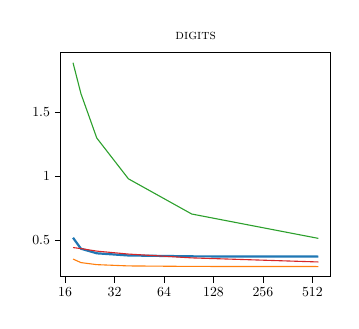
\begin{tikzpicture}[
scale=0.5
]

\definecolor{crimson2143940}{RGB}{214,39,40}
\definecolor{darkgray176}{RGB}{176,176,176}
\definecolor{darkorange25512714}{RGB}{255,127,14}
\definecolor{forestgreen4416044}{RGB}{44,160,44}
\definecolor{steelblue31119180}{RGB}{31,119,180}

\begin{axis}[
tick align=outside,
tick pos=left,
title={\sc digits},
x grid style={darkgray176},
xmin=-8.8, xmax=536.8,
xtick style={color=black},
xtick={-100,0,100,200,300,400,500,600},
xticklabels={0,16,32,64,128,256,512,},
y grid style={darkgray176},
ymin=0.2101, ymax=1.9679,
ytick style={color=black}
]
\addplot [ultra thick, steelblue31119180]
table {%
16 0.516
32 0.43
64 0.394
128 0.377
256 0.37
512 0.368
};
\addplot [thick, darkorange25512714]
table {%
16 0.349
32 0.321
64 0.305
128 0.295
256 0.291
512 0.29
};
\addplot [thick, forestgreen4416044]
table {%
16 1.888
32 1.646
64 1.298
128 0.978
256 0.702
512 0.511
};
\addplot [thick, crimson2143940]
table {%
16 0.439
32 0.431
64 0.411
128 0.388
256 0.358
512 0.326
};
\end{axis}

\end{tikzpicture}

  \end{minipage}
  \hfill
  \begin{minipage}[t]{.16\textwidth}
    \raggedleft
    % This file was created with tikzplotlib v0.10.1.
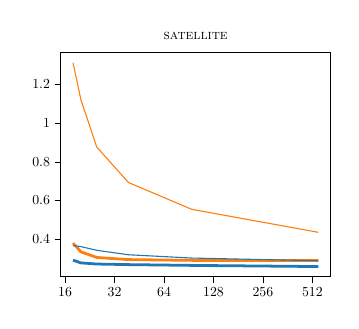
\begin{tikzpicture}[
scale=0.5
]

\definecolor{darkgray176}{RGB}{176,176,176}
\definecolor{darkorange25512714}{RGB}{255,127,14}
\definecolor{steelblue31119180}{RGB}{31,119,180}

\begin{axis}[
tick align=outside,
tick pos=left,
title={\sc satellite},
x grid style={darkgray176},
xmin=-8.8, xmax=536.8,
xtick style={color=black},
xtick={-100,0,100,200,300,400,500,600},
xticklabels={0,16,32,64,128,256,512,},
y grid style={darkgray176},
ymin=0.2053, ymax=1.3647,
ytick style={color=black}
]
\addplot [line width=2pt, darkorange25512714]
table {%
16 0.379
32 0.334
64 0.305
128 0.294
256 0.29
512 0.289
};
\addplot [line width=2pt, steelblue31119180]
table {%
16 0.291
32 0.277
64 0.271
128 0.268
256 0.264
512 0.258
};
\addplot [thick, darkorange25512714]
table {%
16 1.312
32 1.12
64 0.876
128 0.693
256 0.554
512 0.435
};
\addplot [thick, steelblue31119180]
table {%
16 0.367
32 0.361
64 0.342
128 0.319
256 0.302
512 0.288
};
\end{axis}

\end{tikzpicture}

  \end{minipage}\\[-1em]
  %
  % Legend
  \definecolor{steelblue31119180}{RGB}{31,119,180}
  \definecolor{darkorange25512714}{RGB}{255,127,14}
  \newcommand{\myline}[1]{\protect\tikz[baseline=-.5ex,line width=1.6pt]\protect\draw[draw=#1](0,0)--(1.2em,0);}
  \caption{Comparison of convergence in terms of number of inducing points $M$ in NLPD (mean over 10 seeds) on UCI classification tasks: \our (thick) vs.\ subsets (\cite{immer2021improving}, thin). Orange lines (\myline{darkorange25512714}) use the GP mean, whereas blue lines (\myline{steelblue31119180}) the NN MAP estimate as mean. Our \our converges fast for all cases.\looseness-1}
  \label{fig:uci-old}
  %\vspace*{-6pt}
\end{figure}

\begin{table}
  \centering\scriptsize
  \caption{Comparisons and ablations on UCI data with negative log predictive density (NLPD\textcolor{gray}{\footnotesize$\pm$std}, lower better). Our sparse \our ($M=256$) is on par with full models (left) and outperforms the GP subset approach of \cite{immer2021improving} (right). Results for methods marked with * as reported in the original benchmark~\cite{immer2021improving}. See \cref{app:uci} for additional tables with comparisons.}
	\label{tbl:uci-old}
	\vspace*{-4pt}

	% Control table spacing
	\renewcommand{\arraystretch}{1.}
	\setlength{\tabcolsep}{1.2pt}
	\setlength{\tblw}{0.083\textwidth}

	% Custom error formatting
	\newcommand{\val}[2]{%
		$#1$\textcolor{gray}{\tiny ${\pm}#2$}
	}

    % THE TABLE NUMBER ARE GENERATED BY A SCRIPT
	\begin{tabular}{l C{0.6\tblw} C{0.6\tblw} C{0.6\tblw} C{0.6\tblw} C{0.6\tblw} C{0.6\tblw} C{0.6\tblw} C{0.6\tblw} C{0.6\tblw} C{0.6\tblw} C{0.6\tblw} C{0.6\tblw}}
\toprule
& NN MAP & MFVI & BNN & GLM & GLM diag & GLM refine & GLM refine d & SVGP (16) & GP subset(16) & SVGP (32) & GP subset(32)  \\
\midrule
\sc australian & \val{0.31}{0.01} & \val{0.34}{0.01} & \val{0.42}{0.0} & \val{0.32}{0.02} & \val{0.33}{0.01} & \val{0.32}{0.02} & \val{0.31}{0.01} & \val{0.322}{0.028} & \val{0.467}{0.02} & \val{0.316}{0.031} & \val{0.406}{0.016} \\
\sc cancer & \val{0.11}{0.02} & \val{0.11}{0.01} & \val{0.19}{0.0} & \val{0.1}{0.01} & \val{0.11}{0.01} & \val{0.11}{0.01} & \val{0.12}{0.02} & \val{0.102}{0.034} & \val{0.268}{0.012} & \val{0.103}{0.036} & \val{0.206}{0.017} \\
\sc ionosphere & \val{0.35}{0.02} & \val{0.41}{0.01} & \val{0.5}{0.0} & \val{0.29}{0.01} & \val{0.35}{0.01} & \val{0.35}{0.05} & \val{0.32}{0.03} & \val{0.333}{0.041} & \val{0.486}{0.02} & \val{0.313}{0.046} & \val{0.434}{0.025} \\
\sc glass & \val{0.95}{0.03} & \val{1.06}{0.01} & \val{1.41}{0.0} & \val{0.86}{0.01} & \val{0.99}{0.01} & \val{0.98}{0.07} & \val{0.83}{0.02} & \val{0.982}{0.072} & \val{1.225}{0.047} & \val{0.886}{0.082} & \val{1.086}{0.073} \\
\sc vehicle & \val{0.42}{0.007} & \val{0.504}{0.006} & \val{0.885}{0.002} & \val{0.428}{0.005} & \val{0.618}{0.003} & \val{0.402}{0.007} & \val{0.432}{0.005} & \val{0.545}{0.023} & \val{1.001}{0.024} & \val{0.51}{0.021} & \val{0.848}{0.027} \\
\sc waveform & \val{0.335}{0.004} & \val{0.393}{0.003} & \val{0.516}{0.002} & \val{0.339}{0.004} & \val{0.388}{0.003} & \val{0.335}{0.004} & \val{0.364}{0.008} & \val{0.352}{0.024} & \val{0.651}{0.009} & \val{0.343}{0.025} & \val{0.535}{0.017} \\
\sc digits & \val{0.094}{0.003} & \val{0.219}{0.004} & \val{0.875}{0.002} & \val{0.25}{0.002} & \val{0.409}{0.002} & \val{0.15}{0.002} & \val{0.149}{0.008} & \val{0.458}{0.017} & \val{1.724}{0.049} & \val{0.375}{0.015} & \val{1.394}{0.01} \\
\sc satellite & \val{0.23}{0.002} & \val{0.307}{0.002} & \val{0.482}{0.001} & \val{0.241}{0.001} & \val{0.327}{0.002} & \val{0.227}{0.002} & \val{0.248}{0.002} & \val{0}{0} & \val{0}{0} & \val{0.32}{0.013} & \val{0.827}{0.016} \\
\bottomrule
\end{tabular}

\end{table}

% \begin{table}[t!]
%   \centering\scriptsize
%   \caption{Comparisons and ablations on UCI data with negative log predictive density (NLPD\textcolor{gray}{\footnotesize$\pm$std}, lower better). Our sparse \our ($M=256$) is on par with full models (left) and outperforms the GP subset approach of \cite{immer2021improving} (right). Results for methods marked with * as reported in the original benchmark~\cite{immer2021improving}. See App. D.1 for additional tables with comparisons.}
% 	\label{tbl:uci}
% 	\vspace*{-4pt}

% 	% Control table spacing
% 	\renewcommand{\arraystretch}{1.}
% 	\setlength{\tabcolsep}{1.2pt}
% 	\setlength{\tblw}{0.083\textwidth}

% 	% Custom error formatting
% 	\newcommand{\val}[2]{%
% 		$#1$\textcolor{gray}{\tiny ${\pm}#2$}
% 	}

%     % THE TABLE NUMBER ARE GENERATED BY A SCRIPT
% 	% \begin{tabular}{l C{0.6\tblw} C{0.6\tblw} C{0.6\tblw} C{0.6\tblw} C{0.6\tblw} C{0.6\tblw} C{0.6\tblw} C{0.6\tblw} C{0.6\tblw} C{0.6\tblw} C{0.6\tblw} C{0.6\tblw}}
\toprule
& NN MAP & MFVI & BNN & GLM & GLM diag & GLM refine & GLM refine d & SVGP (16) & GP subset(16) & SVGP (32) & GP subset(32)  \\
\midrule
\sc australian & \val{0.31}{0.01} & \val{0.34}{0.01} & \val{0.42}{0.0} & \val{0.32}{0.02} & \val{0.33}{0.01} & \val{0.32}{0.02} & \val{0.31}{0.01} & \val{0.322}{0.028} & \val{0.467}{0.02} & \val{0.316}{0.031} & \val{0.406}{0.016} \\
\sc cancer & \val{0.11}{0.02} & \val{0.11}{0.01} & \val{0.19}{0.0} & \val{0.1}{0.01} & \val{0.11}{0.01} & \val{0.11}{0.01} & \val{0.12}{0.02} & \val{0.102}{0.034} & \val{0.268}{0.012} & \val{0.103}{0.036} & \val{0.206}{0.017} \\
\sc ionosphere & \val{0.35}{0.02} & \val{0.41}{0.01} & \val{0.5}{0.0} & \val{0.29}{0.01} & \val{0.35}{0.01} & \val{0.35}{0.05} & \val{0.32}{0.03} & \val{0.333}{0.041} & \val{0.486}{0.02} & \val{0.313}{0.046} & \val{0.434}{0.025} \\
\sc glass & \val{0.95}{0.03} & \val{1.06}{0.01} & \val{1.41}{0.0} & \val{0.86}{0.01} & \val{0.99}{0.01} & \val{0.98}{0.07} & \val{0.83}{0.02} & \val{0.982}{0.072} & \val{1.225}{0.047} & \val{0.886}{0.082} & \val{1.086}{0.073} \\
\sc vehicle & \val{0.42}{0.007} & \val{0.504}{0.006} & \val{0.885}{0.002} & \val{0.428}{0.005} & \val{0.618}{0.003} & \val{0.402}{0.007} & \val{0.432}{0.005} & \val{0.545}{0.023} & \val{1.001}{0.024} & \val{0.51}{0.021} & \val{0.848}{0.027} \\
\sc waveform & \val{0.335}{0.004} & \val{0.393}{0.003} & \val{0.516}{0.002} & \val{0.339}{0.004} & \val{0.388}{0.003} & \val{0.335}{0.004} & \val{0.364}{0.008} & \val{0.352}{0.024} & \val{0.651}{0.009} & \val{0.343}{0.025} & \val{0.535}{0.017} \\
\sc digits & \val{0.094}{0.003} & \val{0.219}{0.004} & \val{0.875}{0.002} & \val{0.25}{0.002} & \val{0.409}{0.002} & \val{0.15}{0.002} & \val{0.149}{0.008} & \val{0.458}{0.017} & \val{1.724}{0.049} & \val{0.375}{0.015} & \val{1.394}{0.01} \\
\sc satellite & \val{0.23}{0.002} & \val{0.307}{0.002} & \val{0.482}{0.001} & \val{0.241}{0.001} & \val{0.327}{0.002} & \val{0.227}{0.002} & \val{0.248}{0.002} & \val{0}{0} & \val{0}{0} & \val{0.32}{0.013} & \val{0.827}{0.016} \\
\bottomrule
\end{tabular}

% 	\begin{tabular}{lcccccccc}
\toprule
 &  & \sc nn map & \sc bnn & \sc glm & {\sc gp} subset (\sc gp) & \our (\sc gp) \\
Dataset & $M (\%)$ &  &  &  &  &  \\
\midrule
\multirow[t]{10}{*}{Australian (N=690, D=14, C=2)} & 1 & - & - & - & \val{0.68}{0.02} & \val{0.47}{0.08} \\
 & 2 & - & - & - & \val{0.67}{0.02} & \val{0.39}{0.03} \\
 & 5 & - & - & - & \val{0.58}{0.06} & \val{0.36}{0.03} \\
 & 10 & - & - & - & \val{0.51}{0.11} & \val{0.35}{0.03} \\
 & 15 & - & - & - & \val{0.43}{0.04} & \val{0.35}{0.03} \\
 & 20 & - & - & - & \val{0.41}{0.04} & \val{0.35}{0.04} \\
 & 40 & - & - & - & \val{0.38}{0.03} & \val{0.35}{0.03} \\
 & 60 & - & - & - & \val{0.36}{0.04} & \val{0.35}{0.03} \\
 & 80 & - & - & - & \val{0.36}{0.03} & \val{0.35}{0.04} \\
 & 100 & - & - & - & \val{0.35}{0.04} & \val{0.35}{0.04} \\
\cline{1-7}
\multirow[t]{10}{*}{Breast cancer (N=683, D=10, C=2)} & 1 & - & - & - & \val{0.44}{0.03} & \val{0.08}{0.04} \\
 & 2 & - & - & - & \val{0.41}{0.01} & \val{0.09}{0.04} \\
 & 5 & - & - & - & \val{0.43}{0.22} & \val{0.08}{0.04} \\
 & 10 & - & - & - & \val{0.21}{0.06} & \val{0.08}{0.04} \\
 & 15 & - & - & - & \val{0.15}{0.06} & \val{0.08}{0.04} \\
 & 20 & - & - & - & \val{0.13}{0.03} & \val{0.08}{0.04} \\
 & 40 & - & - & - & \val{0.10}{0.04} & \val{0.08}{0.04} \\
 & 60 & - & - & - & \val{0.09}{0.04} & \val{0.08}{0.04} \\
 & 80 & - & - & - & \val{0.09}{0.04} & \val{0.08}{0.04} \\
 & 100 & - & - & - & \val{0.08}{0.04} & \val{0.08}{0.04} \\
\cline{1-7}
\multirow[t]{10}{*}{Digits (N=1797, D=64, C=10)} & 1 & - & - & - & \val{2.10}{0.43} & \val{0.33}{0.07} \\
 & 2 & - & - & - & \val{1.77}{0.71} & \val{0.15}{0.03} \\
 & 5 & - & - & - & \val{0.48}{0.04} & \val{0.10}{0.03} \\
 & 10 & - & - & - & \val{0.33}{0.08} & \val{0.09}{0.03} \\
 & 15 & - & - & - & \val{0.21}{0.02} & \val{0.08}{0.03} \\
 & 20 & - & - & - & \val{0.16}{0.04} & \val{0.08}{0.03} \\
 & 40 & - & - & - & \val{0.10}{0.03} & \val{0.08}{0.03} \\
 & 60 & - & - & - & \val{0.09}{0.03} & \val{0.08}{0.03} \\
 & 80 & - & - & - & \val{0.08}{0.03} & \val{0.08}{0.03} \\
 & 100 & - & - & - & \val{0.08}{0.03} & \val{0.08}{0.03} \\
\cline{1-7}
\multirow[t]{10}{*}{Glass (N=214, D=9, C=6)} & 1 & - & - & - & \val{1.68}{0.09} & \val{1.34}{0.15} \\
 & 1 & - & - & - & \val{1.63}{0.06} & \val{1.27}{0.09} \\
 & 5 & - & - & - & \val{1.45}{0.10} & \val{1.07}{0.10} \\
 & 9 & - & - & - & \val{1.41}{0.16} & \val{0.94}{0.08} \\
 & 15 & - & - & - & \val{1.21}{0.06} & \val{0.92}{0.13} \\
 & 19 & - & - & - & \val{1.19}{0.08} & \val{0.92}{0.11} \\
 & 39 & - & - & - & \val{1.04}{0.08} & \val{0.90}{0.13} \\
 & 59 & - & - & - & \val{0.96}{0.12} & \val{0.87}{0.17} \\
 & 79 & - & - & - & \val{0.91}{0.13} & \val{0.86}{0.13} \\
 & 99 & - & - & - & \val{0.88}{0.14} & \val{0.88}{0.16} \\
\cline{1-7}
\multirow[t]{10}{*}{Ionosphere (N=351, D=34, C=2)} & 1 & - & - & - & \val{0.68}{0.02} & \val{0.47}{0.03} \\
 & 2 & - & - & - & \val{0.69}{0.03} & \val{0.43}{0.05} \\
 & 5 & - & - & - & \val{0.63}{0.05} & \val{0.39}{0.04} \\
 & 10 & - & - & - & \val{0.55}{0.08} & \val{0.39}{0.03} \\
 & 15 & - & - & - & \val{0.46}{0.02} & \val{0.39}{0.04} \\
 & 20 & - & - & - & \val{0.44}{0.03} & \val{0.39}{0.04} \\
 & 40 & - & - & - & \val{0.41}{0.03} & \val{0.39}{0.04} \\
 & 60 & - & - & - & \val{0.41}{0.06} & \val{0.38}{0.04} \\
 & 80 & - & - & - & \val{0.38}{0.04} & \val{0.40}{0.06} \\
 & 100 & - & - & - & \val{0.38}{0.04} & \val{0.40}{0.06} \\
\cline{1-7}
\multirow[t]{10}{*}{Satellite (N=6435, D=35, C=6)} & 1 & - & - & - & \val{1.65}{0.37} & \val{0.37}{0.01} \\
 & 2 & - & - & - & \val{1.14}{0.45} & \val{0.32}{0.02} \\
 & 5 & - & - & - & \val{0.72}{0.02} & \val{0.31}{0.02} \\
 & 10 & - & - & - & \val{0.61}{0.06} & \val{0.30}{0.02} \\
 & 15 & - & - & - & \val{0.52}{0.08} & \val{0.31}{0.04} \\
 & 20 & - & - & - & \val{0.43}{0.05} & \val{0.31}{0.03} \\
 & 40 & - & - & - & \val{0.39}{0.04} & \val{0.30}{0.02} \\
 & 60 & - & - & - & \val{0.35}{0.03} & \val{0.30}{0.02} \\
 & 80 & - & - & - & \val{0.34}{0.04} & \val{0.31}{0.01} \\
 & 100 & - & - & - & - & \val{0.29}{nan} \\
\cline{1-7}
\multirow[t]{10}{*}{Vehicle (N=846, D=18, C=4)} & 1 & - & - & - & \val{1.31}{0.09} & \val{0.96}{0.19} \\
 & 2 & - & - & - & \val{1.15}{0.04} & \val{0.58}{0.02} \\
 & 5 & - & - & - & \val{1.09}{0.23} & \val{0.47}{0.03} \\
 & 10 & - & - & - & \val{0.73}{0.06} & \val{0.45}{0.04} \\
 & 15 & - & - & - & \val{0.63}{0.02} & \val{0.44}{0.04} \\
 & 20 & - & - & - & \val{0.61}{0.06} & \val{0.43}{0.02} \\
 & 40 & - & - & - & \val{0.49}{0.04} & \val{0.43}{0.03} \\
 & 60 & - & - & - & \val{0.45}{0.01} & \val{0.44}{0.02} \\
 & 80 & - & - & - & \val{0.43}{0.04} & \val{0.43}{0.03} \\
 & 100 & - & - & - & \val{0.42}{0.03} & \val{0.42}{0.03} \\
\cline{1-7}
\multirow[t]{10}{*}{Waveform (N=1000, D=21, C=3)} & 1 & - & - & - & \val{0.97}{0.10} & \val{0.33}{0.03} \\
 & 2 & - & - & - & \val{0.74}{0.18} & \val{0.33}{0.03} \\
 & 5 & - & - & - & \val{0.61}{0.24} & \val{0.33}{0.03} \\
 & 10 & - & - & - & \val{0.43}{0.01} & \val{0.32}{0.03} \\
 & 15 & - & - & - & \val{0.38}{0.03} & \val{0.32}{0.03} \\
 & 20 & - & - & - & \val{0.36}{0.03} & \val{0.32}{0.03} \\
 & 40 & - & - & - & \val{0.33}{0.03} & \val{0.32}{0.03} \\
 & 60 & - & - & - & \val{0.32}{0.03} & \val{0.32}{0.03} \\
 & 80 & - & - & - & \val{0.33}{0.03} & \val{0.32}{0.03} \\
 & 100 & - & - & - & \val{0.32}{0.03} & \val{0.32}{0.03} \\
\cline{1-7}
\bottomrule
\end{tabular}

% \end{table}

\clearpage

% \phantomsection%
\addcontentsline{toc}{section}{References}
% \begingroup
\small
\bibliographystyle{abbrvnat}
\bibliography{bibliography}%zotero-library
% \endgroup

\end{document}
